\documentclass[class=minimal,border=0pt]{standalone}
\usepackage{tikz,amsmath, amssymb,bm,color}

\usetikzlibrary{shapes,arrows}
\usetikzlibrary{fit,backgrounds,positioning,calc}
\begin{document}
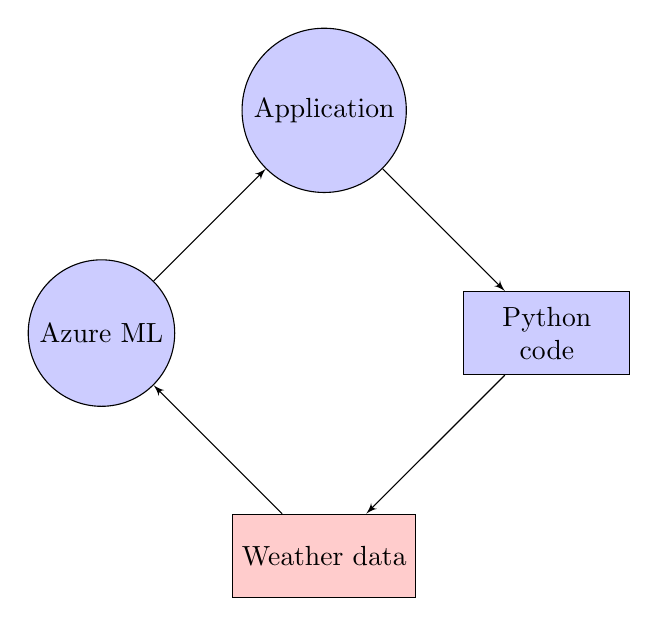
\begin{tikzpicture}[auto, align=center, node distance=4cm, >=latex']

%local definitions
\tikzstyle{DataSource} = [draw, fill=red!20, rectangle,minimum height=3em, minimum width=6em]
\tikzstyle{Client} = [draw, fill=blue!20, rectangle,minimum height=3em, minimum width=6em]
\tikzstyle{Product} = [draw, fill=blue!20, circle]
\tikzstyle{pinstyle} = [pin edge={to-,thin,black}]

\pgfdeclarelayer{background}
\pgfdeclarelayer{foreground}

%main loop
	\node [Product] (Application) {Application};
	\node [Client, below right of=Application] (Python) {Python\\code};
	\node [DataSource, below left of=Python] (DB) {Weather data};
	\node [Product, above left of=DB] (ML) {Azure ML};


	
	%\node [Client, below of=PredictionModel] (lifePrediction) {Live Predictions\\(location \& direction)};


	
	
%connections

	%\draw [->] (Application) -- node[below,midway,fill=white]{Time\\Location} (Python);
	\draw [->] (Application) --  (Python);
	\draw [->] (Python) --  (DB);
	\draw [->] (DB) --  (ML);
	\draw [->] (ML) --  (Application);
	%\draw [thick,->] (PredictionModel) -- node[above,midway,fill=white]{prob} (lifePrediction);



	%block names
	%\node  at ($(PredictionModel -| exData)+(0.5,0.5)$) {SAP HANA};	
	%\node (ClientStart)  at ($(clientPU.north)+(-0.5,0.5)$) {CLIENTS};	
	
%\begin{scope}[on background layer]
%	\filldraw [draw=black,fill=magenta!10,opacity=0.5] ($(PredictionModel -| exData)-(2,-1)$) rectangle ($(lifePrediction.south)+(5,-1)$);
%	\filldraw [draw=black,fill=blue!20,opacity=0.5] ($(ClientStart.north)-(1.8,0)$) rectangle ($(clientGov.south east)+(1,-1.5)$);
	
%\end{scope}




\end{tikzpicture}
\end{document}
